\documentclass[tikz, convert={outfile=\jobname.svg}]{standalone}

\usepackage{tkz-euclide}
\usetikzlibrary{calc}
\usetikzlibrary{decorations.pathreplacing,angles,quotes}
\usetikzlibrary{calligraphy}
\usepackage{xcolor}
\color[rgb]{1,1,1}

\begin{document}
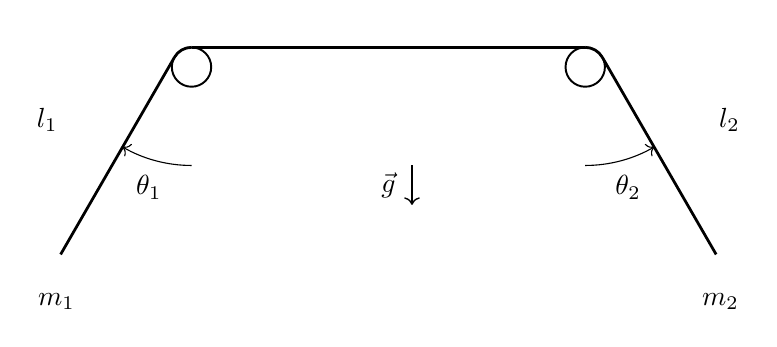
\begin{tikzpicture}
\pgfmathsetmacro{\separation}{5}
\pgfmathsetmacro{\pulleyradius}{0.25}
\pgfmathsetmacro{\massradius}{0.1}
\pgfmathsetmacro{\lengthleft}{3}
\pgfmathsetmacro{\lengthright}{3}
\pgfmathsetmacro{\thetaleft}{30}
\pgfmathsetmacro{\thetaright}{30}
\pgfmathsetmacro{\stringwidth}{1pt}
\pgfmathsetmacro{\pulleywidth}{0.7pt}
\pgfmathsetmacro{\dashedwidth}{0.5pt}


\coordinate (left_pulley) at (-\separation / 2, 0);
\coordinate (right_pulley) at (\separation / 2, 0);
\coordinate (left_touch) at ($(left_pulley) + ({-\pulleyradius * cos(\thetaleft)}, {\pulleyradius * sin(\thetaleft)})$);
\coordinate (right_touch) at ($(right_pulley) + ({\pulleyradius * cos(\thetaright)}, {\pulleyradius * sin(\thetaright)})$);
\coordinate (left_mass) at ($(left_touch) + ({-\lengthleft * sin(\thetaleft)}, {-\lengthleft * cos(\thetaleft)})$);
\coordinate (right_mass) at ($(right_touch) + ({\lengthright * sin(\thetaright)}, {-\lengthright * cos(\thetaright)})$);
\coordinate (l1_node) at ($(left_mass)!0.5!(left_touch) + ({-cos(\thetaleft)}, {sin(\thetaleft)})$);
\coordinate (l2_node) at ($(right_mass)!0.5!(right_touch) + ({cos(\thetaright)}, {sin(\thetaright)})$);

\draw [line width=\stringwidth] (-\separation / 2, \pulleyradius) -- (\separation / 2, \pulleyradius);
\draw [line width=\stringwidth] (left_touch) -- +({-\lengthleft * sin(\thetaleft)}, {-\lengthleft * cos(\thetaleft)});
\draw [line width=\stringwidth] (right_touch) -- +({\lengthright * sin(\thetaright)}, {-\lengthright * cos(\thetaright)});
\draw [line width=\stringwidth] ($(left_pulley) + (0, \pulleyradius)$) arc (90:180-\thetaleft:\pulleyradius);
\draw [line width=\stringwidth] ($(right_pulley) + (0, \pulleyradius)$) arc (90:\thetaright:\pulleyradius);

\draw [line width=\pulleywidth] (left_pulley) circle [radius=\pulleyradius];
% \draw [line width=0.5*\pulleywidth] (left_pulley) circle [radius=0.5*\pulleyradius];
\draw [line width=\pulleywidth] (right_pulley) circle [radius=\pulleyradius];
% \draw [line width=0.5*\pulleywidth] (right_pulley) circle [radius=0.5*\pulleyradius];
\draw (left_mass) [fill=white, white] circle [radius=\massradius];
\draw (right_mass) [fill=white, white]circle [radius=\massradius];
% \draw [decoration={brace, mirror, raise=5pt}, decorate] (left_touch) -- node [below=6pt] {$x$} (left_mass);
\draw [pen colour={white}, fill=white, decoration={calligraphic brace, amplitude=5pt, raise=10pt}, decorate, line width=1pt] (left_mass) -- (left_touch);
\draw [pen colour={white}, fill=white, decoration={calligraphic brace, amplitude=5pt, raise=10pt}, decorate, line width=1pt] (right_touch) -- (right_mass);
\node at (l1_node) {$l_1$};
\node at (l2_node) {$l_2$};
\draw [dashed, line width=\dashedwidth, white] ($(left_pulley) + (0, -\pulleyradius - 0.1)$) -- (left_pulley |- left_mass);
\draw [dashed, line width=\dashedwidth, white] ($(right_pulley) + (0, -\pulleyradius - 0.1)$) -- (right_pulley |- right_mass);
% \draw [dashed] let \p1 = (left_mass) in (left_pulley) -- (0, \y1);
\coordinate (left_pulley_mass) at (left_pulley |- left_mass);
\coordinate (right_pulley_mass) at (right_pulley |- right_mass);
% \path [name intersection]
\tkzInterLL(left_mass,left_touch)(left_pulley_mass,left_pulley) \tkzGetPoint{left_pivot};
\tkzInterLL(right_mass,right_touch)(right_pulley_mass,right_pulley) \tkzGetPoint{right_pivot};
\pic [draw, <-, "$\theta_1$", angle eccentricity=1.2, angle radius=1.75cm] {angle=left_mass--left_pivot--left_pulley_mass};
\pic [draw, ->, "$\theta_2$", angle eccentricity=1.2, angle radius=1.75cm] {angle=right_pulley_mass--right_pivot--right_mass};
\node (gravity) at (0, -1.5) {$\vec{g}$} [right];
\draw [->, line width=0.5pt] ($(gravity) + (0.3, 0.25)$) -- ($(gravity) + (0.3, -0.25)$);
\node at (left_mass) [below=8pt] {$m_1$};
\node at (right_mass) [below=8pt] {$m_2$};
\end{tikzpicture}
\end{document}
